\begin{exercice*}
    Groot réalise les motifs suivants en mosaïque.
    \smallskip
    \begin{minipage}{0.2\linewidth}
        \begin{center}
            {\bfseries Motif 1}\\\smallskip
            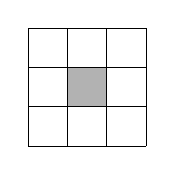
\begin{tikzpicture}[scale = 0.5]                        
                \fill[color=black!30] (1,1)--(2,1)--(2,2)--(1,2)--cycle;
                \draw[help lines, color=black] (0,0) grid (3,3);
            \end{tikzpicture}
        \end{center}
    \end{minipage}
    \begin{minipage}{0.3\linewidth}
        \begin{center}
            {\bfseries Motif 2}\\\smallskip
            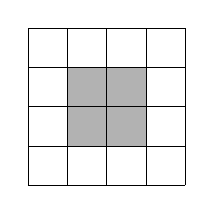
\begin{tikzpicture}[scale = 0.5]                        
                \fill[color=black!30] (1,1)--(3,1)--(3,3)--(1,3)--cycle;
                \draw[help lines, color=black] (0,0) grid (4,4);
            \end{tikzpicture}
        \end{center}
    \end{minipage}
    \begin{minipage}{0.2\linewidth}
        \begin{center}
            {\bfseries Motif 3}\\\smallskip
            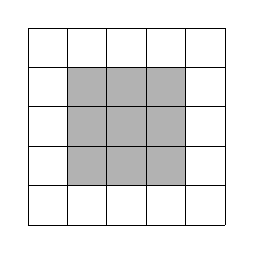
\begin{tikzpicture}[scale = 0.5]                        
                \fill[color=black!30] (1,1)--(4,1)--(4,4)--(1,4)--cycle;
                \draw[help lines, color=black] (0,0) grid (5,5);
            \end{tikzpicture}
        \end{center}
    \end{minipage}

    Il forme un carré avec des carreaux gris, puis le borde avec des carreaux blancs.
    \begin{enumerate}
        \item Déterminer le nombre de carreaux blancs nécessaires pour réaliser le {\bfseries motif 4}.
        \item Justifier que Groot peut réaliser un motif de ce type avec \num{144} carreaux gris.
        \item Déterminer alors le nombre de carreaux blancs nécessaires.
        \item On appelle {\bfseries motif $\boldsymbol{n}$} le motif contenant {\bfseries $\boldsymbol{n}$} carreaux gris. Pier, Pol et Jak ont chacun proposé une expression
        pour calculer le nombre de carreaux blancs nécessaires :
        \begin{description}
            \item[Expression n°1 : ] $2\times n + 2\times(n+2)$
            \item[Expression n°2 : ] $2\times n + 2\times(n+2)$
            \item[Expression n°3 : ] $2\times n + 2\times(n+2)$
        \end{description}
        Déterminer la seule expression qui ne convient pas.
    \end{enumerate}
\end{exercice*}
\begin{corrige}
    %\setcounter{partie}{0} % Pour s'assurer que le compteur de \partie est à zéro dans les corrigés
    %\phantom{rrr}    
    Groot réalise les motifs suivants en mosaïque.
    \smallskip
    \begin{minipage}{0.2\linewidth}
        \begin{center}
            {\bfseries Motif 1}\\\smallskip
            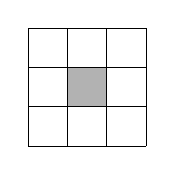
\begin{tikzpicture}[scale = 0.5]                        
                \fill[color=black!30] (1,1)--(2,1)--(2,2)--(1,2)--cycle;
                \draw[help lines, color=black] (0,0) grid (3,3);
            \end{tikzpicture}
        \end{center}
    \end{minipage}
    \begin{minipage}{0.3\linewidth}
        \begin{center}
            {\bfseries Motif 2}\\\smallskip
            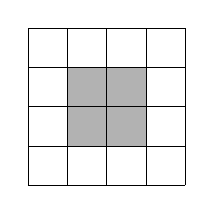
\begin{tikzpicture}[scale = 0.5]                        
                \fill[color=black!30] (1,1)--(3,1)--(3,3)--(1,3)--cycle;
                \draw[help lines, color=black] (0,0) grid (4,4);
            \end{tikzpicture}
        \end{center}
    \end{minipage}
    \begin{minipage}{0.2\linewidth}
        \begin{center}
            {\bfseries Motif 3}\\\smallskip
            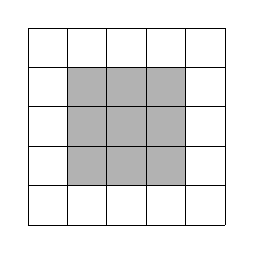
\begin{tikzpicture}[scale = 0.5]                        
                \fill[color=black!30] (1,1)--(4,1)--(4,4)--(1,4)--cycle;
                \draw[help lines, color=black] (0,0) grid (5,5);
            \end{tikzpicture}
        \end{center}
    \end{minipage}

    Il forme un carré avec des carreaux gris, puis le borde avec des carreaux blancs.

    \begin{enumerate}
        \item Déterminer le nombre de carreaux blancs nécessaires pour réaliser le {\bfseries motif 4}.\\
        {\red 4 carreaux gris donc $6^2-4^2$ carreaux blancs, soit $20$. Groot utilisera $20$ carreaux blancs.}
        \item Justifier que Groot peut réaliser un motif de ce type avec \num{144} carreaux gris.\\
        Puisque $144=12^2$, on peut faire un motif avec $12$ carreaux gris. C'est le {\bfseries motif 12}.
        \item Déterminer alors le nombre de carreaux blancs nécessaires.\\
        {\red Comme $14^2-12^2=196-144=52$, il faudra donc $52$ carreaux blancs.}
        \item On appelle {\bfseries motif $\boldsymbol{n}$} le motif contenant {\bfseries $\boldsymbol{n}$} carreaux gris. Pier, Pol et Jak ont chacun proposé une expression
        pour calculer le nombre de carreaux blancs nécessaires :\\
        \begin{itemize}
            \def\item{}
            \item {\bfseries Expression n°1 : }$2\times n + 2\times(n+2)$\\
            \item {\bfseries Expression n°2 : }$2\times n + 2\times(n+2)$\\
            \item {\bfseries Expression n°3 : }$2\times n + 2\times(n+2)$\\
        \end{itemize}
        Déterminer la seule expression qui ne convient pas.\\
        {\red Pour un motif de {\bfseries $\boldsymbol{n}$} carreaux gris, il faut $(n+2)^2-n^2=n^2+4n+4-n^2=4n+4$ or l'expression n°2 vaut $4n+8$ donc elle ne convient pas.}
    \end{enumerate}
\end{corrige}

